\startchapter{Multi-Hop Transmission}
\label{chapter:multi}

As new IoT applications emerge, the need for reliable multi-hop transmission between sensors is becoming more and more obvious. In many sensor network applications data can not be gathered using a single sink node and it has to be relayed with the help of other nodes. Linear sensor networks are one of the main applications with this criteria. They can be used for monitoring long highways, railroads, skyscrapers and walls. In many of these applications using wire to connect sensors is either simply impossible or very expensive to deploy and maintain.

Multi-hop relaying has always been a bottle neck for wireless communications. As the number of hops grows, the end to end throughput suffers drastically. A significant research effort has been employed to improve the throughput and reliability of multi-hop transmissions. Recognizing interference as the main obstacle in multi-hop transmission, many new technologies have emerged. Technologies such as successive interference cancellation \cite{alvandi2015delay}, multi-packet detection and collision resolution using zigzag \cite{mzig}, interference alignment \cite{4567443, 7218598}, and full-duplex (FD) radios \cite{fullduplex} have all tried to use interference and broadcast nature of wireless channel in their favor.

One of the technologies that is promising for multi-hop sensor network applications is physical layer network coding. It can increase the end to end throughput by decreasing the number of time slots that are required for a multi-hop transmission while maintaining an acceptable error rate. In the following sections, first the concept of PNC is explained and then our contribution is elaborated.

\section{Physical Layer Network Coding}

The concept of Network Coding is nothing new in the wireless domain. It relies on optimizing transmission of data by combining two or more messages in a network. Physical Layer Network Coding(PNC) is then nothing but a network coding happening at the physical layer.

We use a three node linear network example to illustrate this idea \cite{zhang2006hot}. In figure \ref{fig:justThreeNodes}, nodes $A$ and $B$ have packets to exchange and node $R$ can act as a relay.


\begin{figure}
    \centering
    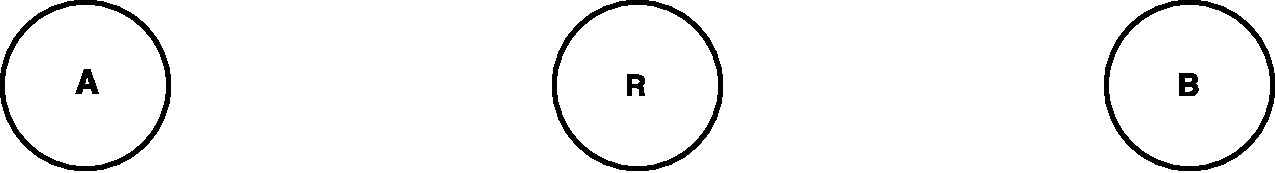
\includegraphics[width=0.8\textwidth]{figures/justThreeNodes.pdf}
    \caption{Simple three node linear network. Nodes $A$ and $B$ have packets to exchange and node $R$ acts as relay} \label{fig:justThreeNodes}
\end{figure}

Assuming that $A$ and $B$ are too far for a reliable transmission, there are different ways for this exchange of packets to happen, traditional relaying, straightforward network coding and physical layer network coding.

An exchange of packets between $A$ and $B$ where relay only works as a traditional decode and forward node takes four time slots as illustrated in figure \ref{fig:traditionalRelay}.  

\begin{figure}
    \centering
    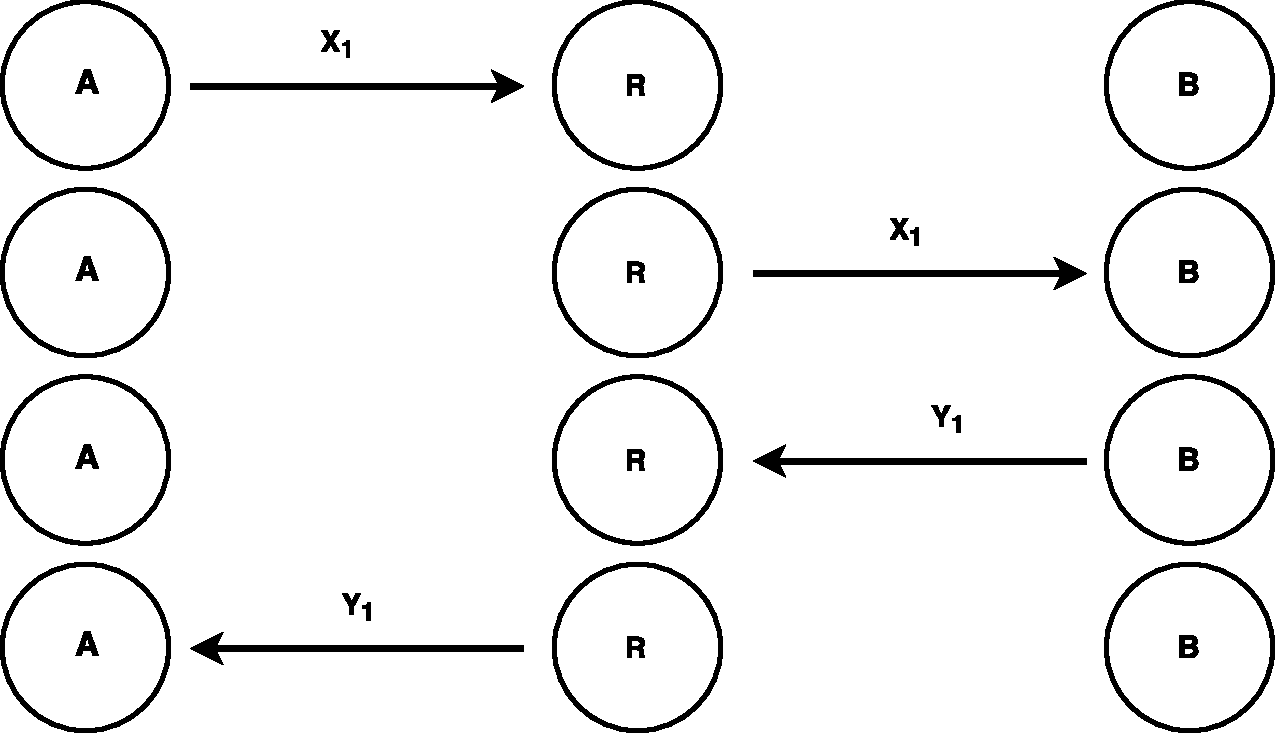
\includegraphics[width=0.8\textwidth]{figures/traditionalRelay.pdf}
    \caption{Traditional relaying. First, node $A$ transmits its packet to the relay, then the relay forwards $A$'s packet to $B$, then in time slot three, node B sends its packet to the relay, which is then forwarded to node $A$ in time slot four.} \label{fig:traditionalRelay}
\end{figure}

Using straightforward network coding, reduces the number of time slots required for that aforementioned exchanged to happen to three. Figure \ref{fig:straightforwardNC} shows this scenario. This way, using the broadcast nature of the wireless channel, the relay having stored both $A$ and $B$'s message, broadcasts a combined version of $X_1$ and $Y_1$. Then both $A$ and $B$ can decode the other node's packet, having their own message and the message they received from the relay. The simplest coding scheme to be used by relay to generate the combined message is calculating XOR of  $X_1$ and $Y_1$.

\begin{figure} 
    \centering
    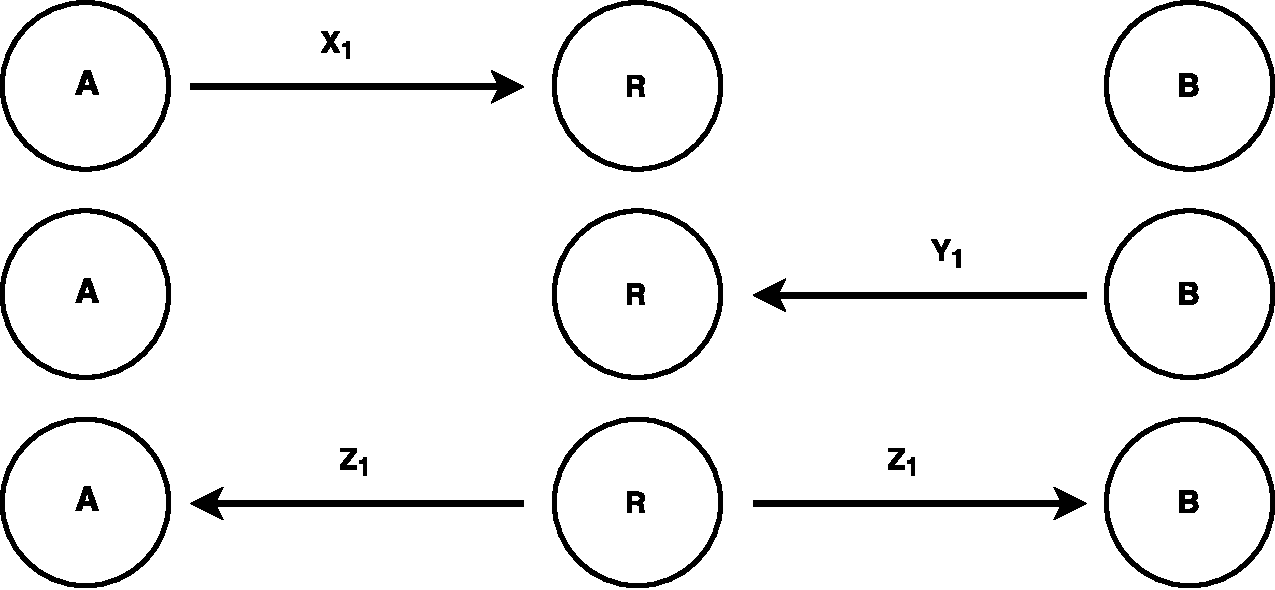
\includegraphics[width=0.8\textwidth]{figures/straightforwardNC.pdf}
    \caption{Straightforward network coding. First, $A$ transmits its packet to relay, then $B$ transmits its message to the relay, then relay calculates $Z_1=X_1 \oplus Y_1$ and broadcasts it to $A$ and $B$ in time slot three, which can then decode the other nodes message by another XOR.} \label{fig:straightforwardNC}
\end{figure}

\begin{figure}
    \centering
    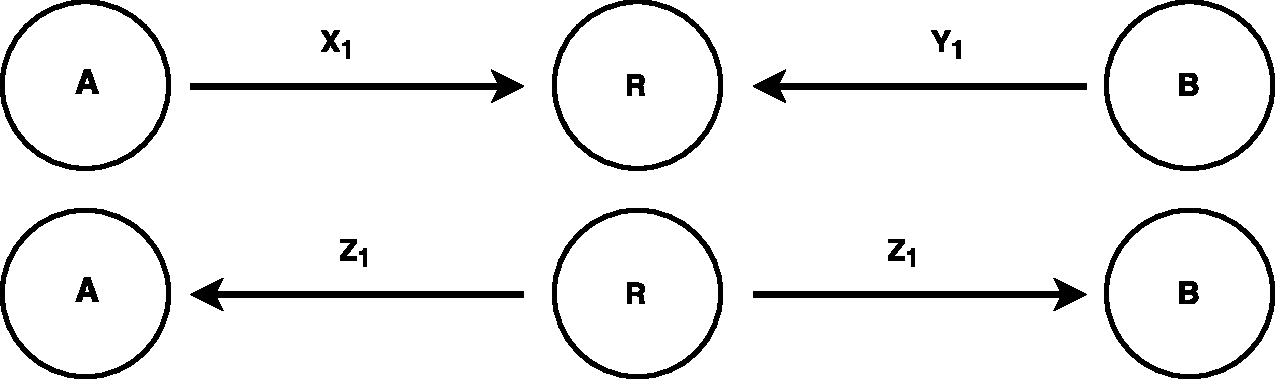
\includegraphics[width=0.8\textwidth]{figures/threeNodePnc.pdf}
    \caption{Physical layer network coding. In time slot one, $A$ and $B$ will transmit their packets to the relay at the same time (multiple access phase). The relay, using its mapping function extracts XOR of $A$ and $B$'s packets and broadcasts it to them in time slot two (broadcast phase).} \label{fig:threeNodePnc}
\end{figure}

Physical layer network coding is similar to straightforward networking coding with the difference that in PNC, the two messages from $A$ and $B$ are coded (combined) in the physical layer using the additive nature of simultaneously arriving electromagnetic (EM) waves \cite{zhang2006hot}. This reduces the number of time slots for the same exchange to happen to two. In a simple BPSK modulation where 0 and 1 are represented with $-1$ and $+1$ respectively, if $A$ and $B$ transmit their packet to the relay at the same time, they relay will received symbols of $-2$, $0$, and $+2$. At this step, every PNC capable relay requires a mapping function, to convert these new symbols into bits of data with a meaningful relationship to $A$ and $B$'s bits. In this simple BPSK example, mapping $-2$ and $+2$ symbols to 1 and $0$ symbols to 0, means that the received message at the relay is again XOR of $A$ and $B$'s packets. Just like the straightforward network coding, the relay then broadcasts this information back to $A$ and $B$ and they will use it to extract the other node's packet.

The same technique can be extended to linear multi-hop networks with more than two hops. Although a multi-hop scenario suffers from interference from other nodes, PNC is among technologies that can still maintain a reliable error rate and much higher throughput.

While the theory of PNC technology has been around for a while, it's implementation and real-life applications have lacked behind. A practical PNC implementation has multiple challenges, most notably Carrier-Frequency Offsets (CFO) and timing synchronization. In the Multiple Access (MA) phase, the relay has to receive a signal from two sources, tracking the CFO from two transmitters while their signals is superimposed is one of the main difficulties. Existing implementations require an interference free part in each signal which comes with a high overhead and is restrictive for multi-hop scenarios. This thesis proposes a novel idea to overcome the CFO challenge and have the relay correctly receive the sum signal in MA phase. The following sections explain design and implementation of a Software Defined Radio (SDR) PNC communication system on the GNURadio platform. The design is then implemented on USRP testbed. Extensive simulations and experiments have been done to investigate the proposed implementation and its feasibility. The results are presented in chapter \ref{chapter:eval}.

\section{Implementation}
We implemented the proposed MPNC on USRP and GNURadio to build the multi-hop wireless testbed.
% This section presents the details of our implementation. There are two types of transmissions in the system, the multi-access (MA) transmission and the single-hop transmission. 
For MPNC, the transmitter and receiver in the single-hop transmission can be made using regular transmission and reception chains. In this work, standard BPSK blocks of GNURadio are used for all steps of communication, modulation, timing recovery, phase tracking and demodulation.

%The MA transmission, on the other hand, has several challenges that should be addressed and solved carefully.   Different from point-to-point transmissions or asynchronous packet collisions, in MPNC, signals with different carrier frequency offsets (CFOs) are superimposed at the receiver simultaneously, the estimation and compensation of CFOs becomes much more challenging. Although PNC has been a hot topic in the past decade, the implementation work is very limited. In~\cite{lu2013implementation}, PNC was implemented where the mean of the two CFOs was used for compensation. In multi-hop scenario, the error propagation is a severer problem than that in the two-hop PNC case,  so a careful design that can accurately compensate the CFOs is needed.
For  MA transmissions, signals from two transmitters are synchronized in the symbol level. The synchronization issue has been heavily investigated, e.g.,
SourceSync~\cite{sourcesync} can achieve low-overhead distributed synchronization with the accuracy of tens of $ns$, 
smaller than the symbol duration (e.g., 802.11 OFDM symbol time of 4 $\mu$s).
%such as  using GPS receiver in outdoor environment, or various synchronization protocols wherever the GPS signal is not available. Also, using OFDM technology can also prolong the symbol duration and make the symbol level synchronization simpler~\cite{lu2013implementation}. 
 %As long as the nodes are synchronized, the assumption of having an equal distance between all transmitters to the relay can be removed by measuring the propagation time difference and offset it when the transmissions are initiated. 
 As synchronization for a static TDMA network is relatively easy and it in fact makes the estimation and compensation of CFOs and detection of preamble during the MA transmission more difficult, we use a MIMO cable to synchronize the transmitters in our USRP testbed, and focus on the most challenging part,  the receiver of MA transmission with symbol level synchronization.

%Different from point-to-point transmissions or asynchronous packet collisions, in MPNC, signals with different carrier frequency offset are superimposed at the receiver simultaneously, which makes the estimation and compensation of carrier frequency offset and detection of preamble extremely challenging. Our solutions to these challenges are presented in this section.
%The challenges and our solutions used in the testbed are presented below.

%\begin{figure}
%    \centering
%    \includegraphics[width=0.4\textwidth]{figure/ma_phase}
%    \caption{A generic MA transmission consists of two nodes transmitting to a relay at the same time}\label{ma_phase}
%\end{figure}


\subsection{Signal formulation}
Since the oscillator at the mixer of practical devices is never perfect, the real carrier frequency of each device may be slightly different from the nominal value. This causes a small rotating phase to remain in the signal after the mixer. In regular point-to-point communications,  this frequency offset can be estimated and compensated using phase tracking algorithms. The same algorithms are no longer useful in MA transmissions since the signals are from two sources and there are two frequency offsets, so the resulting phase cannot be removed by a simple multiplication. 
Several algorithms have been proposed \cite{lu2013implementation,katti2007embracing, gollakota2008zigzag, fung2010preamble} to compensate the effect of CFO when multiple signals are mixed at the receiver. These algorithms either require a small portion of interference-free part in two signals, which are not directly applicable for MPNC with symbol level synchronization. Another approach is to use the mean of two frequency offsets to partially compensate the frequency offsets for PNC MA transmission \cite{lu2013implementation}. In multi-hop scenarios, error propagation is a severer problem than that in the two-hop PNC case,  so a careful design that can accurately compensate the two CFOs is needed.
%Obviously, these existing solutions are not directly applicable for MPNC with symbol level synchronization, and we investigated the problem and proposed our own solution. 
%Different from these algorithms, our proposed method does not require any interference free part in two signals, and it does not use the mean of two frequency offsets to only partially compensate the frequency offsets.

Assuming that nodes A and B are transmitting symbol $a_k$ and $b_k$ at the $k_{th}$ symbol interval, respectively, the baseband signal can be written as
\begin{eqnarray}
    x(t)&=&\sum_{k=0}^{k=N} a_k g(t-kT), {\rm \ \ \ \ \ and}\\
    y(t)&=&\sum_{k=0}^{k=N} b_k g(t-kT),
\end{eqnarray}
respectively, where $g(t)$ is the pulse for the pulse shaping step (a root raised cosine (RRC) pulse is used here), $N$ is the number of symbols in one packet, and $T$ is the symbol interval. Considering the received signal as
\begin{equation}
    r(t)=x(t- \tau) H_a e^{j2\pi (f_a)t} + y(t - \tau) H_b e^{j2\pi (f_b)t},
\end{equation}
where $f_a$ ($f_b$) is the CFOs between the oscillator of the receiver and  that of A (B), respectively, and $\tau$ is the time delay. In the MA transmission, $f_a$ and $f_b$ can be estimated at the beginning of each packet. Considering the wireless channels to be frequency flat and constant during the reception time of a packet, %and small bandwidth of BPSK signal, 
$H_a$ ($H_b$) can be represented with one tap, essentially a complex number. The received signal after the Analog to Digital Converter (DAC) is given by
\begin{equation}
    r_n=h_1 x e^{j \omega_1 n + \phi_1} + h_2 y e^{j \omega_2 n + \phi_2},
\end{equation}
where $h_i$, $\phi_i$, and $\omega_i$, $i=1,2$ are the gains, phases and digital frequency offsets imposed by the channel and  the receiver circuit, respectively. 

\subsection{Timing recovery}

Depending on the sampling rate of the Digital to Analog Converter (DAC), each symbol is represented with a constant number of samples. This parameter is called Samples per Symbol ($SpS$) and can be found as ${T}{f_s}$, where $f_s$ is  the sample rate of the DAC. After passing the received signal from the matched filter, the next step is to down sample the signal to one sample per symbol before detection. 

In the digital domain, depending on the offset between the transmitter and receiver's clocks, only one of the samples representing a symbol is used for detection and the distance between valid samples is equal to $SpS$. As shown in Fig.~\ref{fig:pncreceiver}, to find the valid sample, the signal is divided into different branches and decimated with different time delays, from $0$ to $ SpS -1$. The signal after downsampling can be expressed as
\begin{equation}
    s_k=h_1 a_k e^{j (SpS) \omega_1 n + \phi_1} + h_2 b_k e^{j (SpS) \omega_2 n + \phi_2}.
\end{equation}
Each branch is then used for preamble detection purposes and the result is connected to a switch. The same preamble detection algorithm is ran for all branches. If a preamble is identified, the signal would be annotated with a tag consisting of $\phi_i$ and $\omega_i$ ($i=1,2$). The switch then copies only the branch with a tag to output. It is possible to find a preamble in more than one branch. The preamble detector block  also includes the mean square error of detection so the switch can choose the branch with the best signal to noise ratio. %Valid samples can then be expressed as
%c: mohammad: incomplete sentence above. 



\begin{figure}
    \centering
    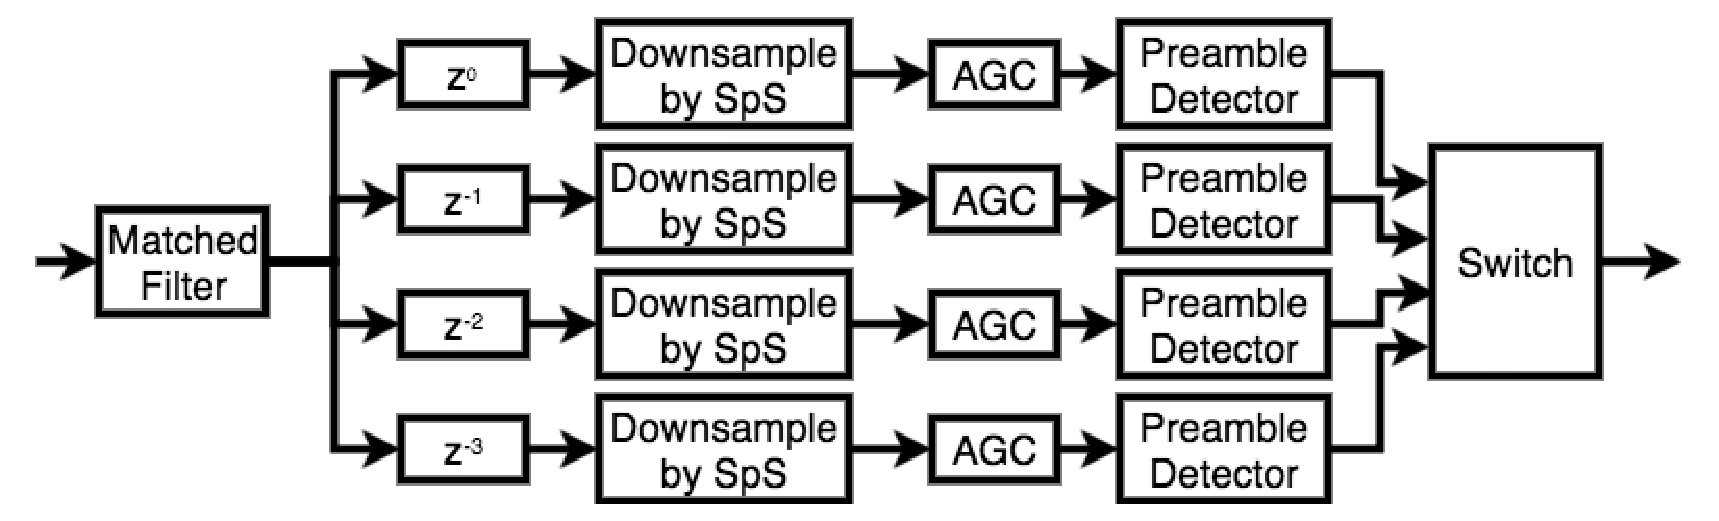
\includegraphics[width=0.95\textwidth]{figures/pncreceiver.eps}
    \caption{Receiver chain.} \label{fig:pncreceiver}
\end{figure}


\subsection{MA receiver, CFO estimation}
To help the receiver estimate CFOs and detect MA transmissions, each frame begins with a Sync preamble and a start of frame delimiter (SFD) part. The sync preamble is a series of zeros and ones, and the SFD is used to verify the detection of a packet.  
%The sync parts are shown in Fig.~\ref{syncs}. 
In our work, the Sync preambles for node A and B are ``1010... 10" and ``0101...01", respectively, which is similar to the packet structure used in the IEEE 802.11 FH PHY.

%\begin{figure}
%    \centering
%    \includegraphics[width=0.3\textwidth]{figure/packet}
%    \caption{Multiple access phase packet structure}\label{ma_packet}
%\end{figure}

Before using the signal to detect a preamble, the signal is passed from an Automatic Gain Control (AGC) unit, in order to normalize the channel gains, $h_1$ and $h_2$.  In a window with a large enough number of symbols, there exists at least one instant that symbols from both sources has an equal or very close phase and have been added constructively. So the AGC adjusts the maximum absolute value of symbols to two. For BPSK,  +1 and -1 represents 1 and 0, respectively. If we index all symbols of the sync part starting from 0, the $k_{th}$ received symbols of Sync preamble can be written as
\begin{equation} \label{maineq}
    s_k=(-1)^{k+1}e^{p_{1,k}} - (-1)^{k}e^{p_{2,k}}.
\end{equation}
For  consistency, we replace all odd indexed symbols of Sync with their additive inverse so the $k_{th}$ symbol can be represented as
%c: mohammad: I cannot understand the above sentence "with their additive inverse..."
\begin{equation}
    s_k^\prime=e^{p_{1,k}} - e^{p_{2,k}}.
\end{equation}
The two phases of $p_{1,k}$ and $p_{2,k}$ can be found by solving the equations below
\begin{equation}
\begin{cases}
    Re(s_k^\prime)=\cos(p_{1,k}) - \cos(p_{2,k}), \\
    Im(s_k^\prime)=\sin(p_{1,k}) - \sin(p_{2,k}).
\end{cases} 
\end{equation}
Since there may be multiple possible answers for these equations,  $p_{1,k}$ and $p_{2,k}$ are chosen in a way that they are closest to $p_{1,k-1}$ and $p_{2,k-1}$ and increasing or decreasing linearly. 

%%%%%%%%%%%%%%%%%%%%%%%%%%%%%%%%%%%%%%%%%%%%%%%%%%%%%%%%%%%%%%%%%%%%%%%%%%%
\iffalse
\begin{equation}
\begin{cases}
    Re(r_i)=-2\sin \left( \frac{p_{1,i}+p_{2,i}}{2}\right)  \sin \left( \frac{p_{1,i}-p_{2,i}}{2}\right), \\
    Im(r_i)=2\sin \left( \frac{p_{1,i}-p_{2,i}}{2}\right)   \cos \left( \frac{p_{1,i}+p_{2,i}}{2}\right).
\end{cases} 
\end{equation}
Then representing $\sin \left( \frac{p_{1,i}+p_{2,i}}{2}\right)$ with $x_{1,i}$ and $\sin \left( \frac{p_{1,i}-p_{2,i}}{2}\right)$ with $x_{2,i}$ we can simplify equations as:

\begin{equation}
    x_{1,i}= \pm \sqrt{\frac{Re^2(r_i)}{Re^2(r_i) + Im^2(r_i)}},
\end{equation}

\begin{equation}
    x_{2,i}= - \frac{Re(r_i)}{2x_{1,i}}.
\end{equation}

the phases can then be found as:
\begin{equation}
    \begin{cases}
        p_{1,i}=k_{1,i} + k_{2,i},\\
        p_{2,i}=k_{1,i} - k_{2,i},\\
    \end{cases}
\end{equation}
where
\begin{equation}
    \begin{cases}
        k_{1,i}= \sin^{-1}(x_{1,i}) \quad or \quad \pi - \sin^{-1}(x_{1,i}), \\
        k_{2,i}= \sin^{-1}(x_{2,i}) \quad or \quad \pi - \sin^{-1}(x_{2,i}),
    \end{cases}
\end{equation}

which leaves four possibilities for answers, each can be tried in (\ref{maineq}) to find the one that matches. 

\fi
%%%%%%%%%%%%%%%%%%%%%%%%%%%%%%%%%%%%%%%%%%%%%%%%%%%%%%%%%%%%%%%%%%%%%%%%%%%

The frequency and phase offsets are then found by a solving a linear regression according to the following equations,
\begin{equation}
    \begin{cases}
        p_{1,k}=(SpS) \omega_1 k + \phi_1, \\
        p_{2,k}=(SpS) \omega_2 k + \phi_2.
    \end{cases}
\end{equation}
\iffalse
where $p_{1,i}^{\prime}$ and $p_{2,i}^{\prime}$ are unwrapped versions of  $p_{1,i}$ and $p_{2,i}$, respectively.
\fi
%
%\begin{figure}
%    \centering
%    \includegraphics[width=0.3\textwidth]{figure/syncs}
%    \caption{Sync preambles. (a) Sync preamble sent by node A . (b) Sync preamble sent by node B}\label{syncs}
%\end{figure}
%
%
%\begin{figure}
%    \centering
%    \includegraphics[width=0.3\textwidth]{figure/sfds}
%    \caption{SFDs. (a) SFD preamble sent by node A. (b) SFD preamble sent by node B. (c) SFD preamble expected in the relay} \label{fig:sfd}
%\end{figure}

\subsection{MA receiver, preamble detection}
A window with the length of the Sync preamble is always sliding on the received samples. Then each time the above CFO estimation algorithm is applied and the $\phi_i$ and $\omega_i$ ($i=1,2$) are used to decode the next $L_{SFD}$ symbols of the packet where $L_{SFD}$  is the length of the SFD part. If the decoded SFD matches the expected SFD, which is XOR of SFD of node A and node B, %Fig. \ref{fig:sfd} (c),
 then the packet is detected and the rest of the symbols are decoded using the same parameters. In our design, SFDs by nodes A  and B are ``1010 0110 1101 0110" and ``1010 1010 0110 1011", respectively, so the SFD expected in the relay is ``0000 1100 1011 1101". 
 
Because of the presence of CFO and phase offset, the constellation is changing from one symbol to another. The right constellation for each received symbol is calculated using the $\phi_i$, and $\omega_i$ and then used for decoding and mapping, According to the mapping function. % as shown in Fig.~\ref{fig:pnc}.
\iffalse you might need to add stuff about the mapping function.\fi
